\section{Results}

\subsection{Pruning via Skeletonization}

\begin{table}
	\centering
	\small
	\begin{tabular}{c c c} \hline
		\textbf{Dataset} & \textbf{Baseline} & \textbf{After Pruning} \\ \hline
		Kasthuri Vol. 1 & 763 / 21242 (3.47\%) & 753 / 3459 (17.88\%) \\
		Kasthuri Vol. 2 & 1010 / 26073 (3.73\%) & 904 / 4327 (17.28\%) \\
		FlyEM Vol. 1 & 269 / 14875 (1.78\%) & 262 / 946 (21.69\%) \\
		FlyEM Vol. 2 & 270 / 16808 (1.58\%) & 285 / 768 (27.07\%)\\ \hline
	\end{tabular}
	\caption{The results of our pruning heuristic compared to the current baseline.}
	\label{table:skeletonization}
\end{table}

Table \ref{table:skeletonization} shows the results of pruning using the skeletonization heuristic.
The baseline algorithm considers all adjacent regions for merging. 
Our method removes a significant portion of these candidates while maintaining a large number of the true merge locations.
This edge pruning is essential for the graph partitioning algorithm which has a computational complexity dependence on the number of edges. 
Our pruning heuristic removes at least $6\times$ the number of edges between correctly split segments on all datasets, achieving a maximum removal ratio of $20\times$. 
Equally important is the number of split errors that remain after pruning.
These are the locations that we want to merge to create a more accurate reconstruction.
For every dataset, the number of positive candidates remains relatively even. 
However, since our heuristic does not enforce an adjacency constraint of two regions when constructing edges in the graph, the difference does not indicate the number of examples excluded by pruning. 
In fact, our method finds a number of examples which are non-adjacent.
Figure \ref{fig:skeleton-results} shows two example segments which are split errors.
The top example our algorithm missed but the segments are adjacent. 
The bottom example our algorithm found despite the fact that they are not adjacent.

\begin{figure}[t!]
	\centering
	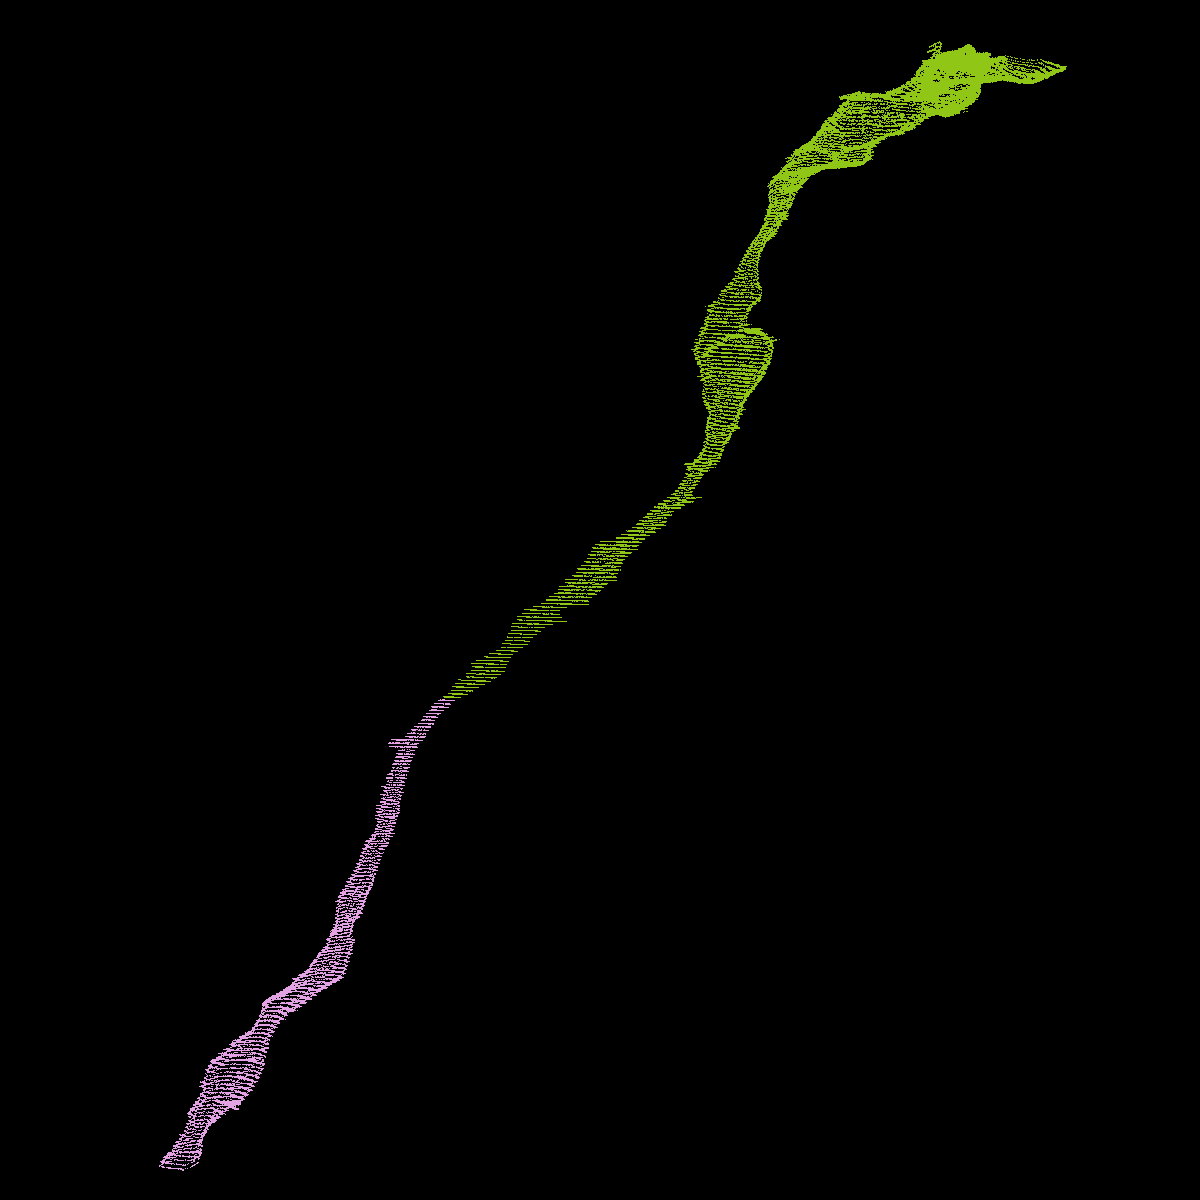
\includegraphics[width=0.85\linewidth]{./figures/merge_candidate1.png}
	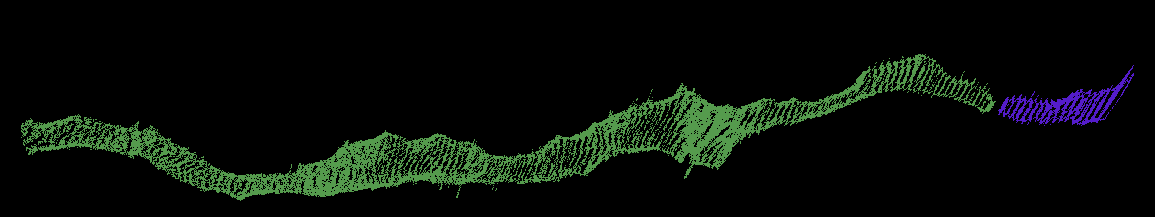
\includegraphics[width=0.85\linewidth]{./figures/merge_candidate2.png}
	\caption{Example merge candidates.}
	\label{fig:skeleton-results}
\end{figure}


\subsection{Classification Performance}

\begin{table}
	\centering
	\begin{tabular}{c c c c} \hline
	\textbf{Dataset} & \textbf{Precision} & \textbf{Recall} & \textbf{Accuracy} \\ \hline
	Kasthuri Training & 0.919 & 0.936 & 0.974 \\
	Kasthuri Testing & 0.737 & 0.717 & 0.907 \\
	FlyEM Vol. 1 & 0.796 & 0.478 & 0.862 \\ 
	FlyEM Vol. 2 & 0.762 & 0.422 & 0.810 \\ \hline
	\end{tabular}
	\caption{Precision and recall for the training and three test datasets.}
	\label{table:classification}
\end{table}

Table \ref{table:classification} shows the precision and recall for all of the datasets. 
Since, our method does not rely on the image data, we can train the network on an anisotropic dataset and get impressive results on an isotropic dataset. 
Figure \ref{fig:network-results} shows the receiver operating characteristic (ROC) curve for all four datasets. 

\begin{figure}
	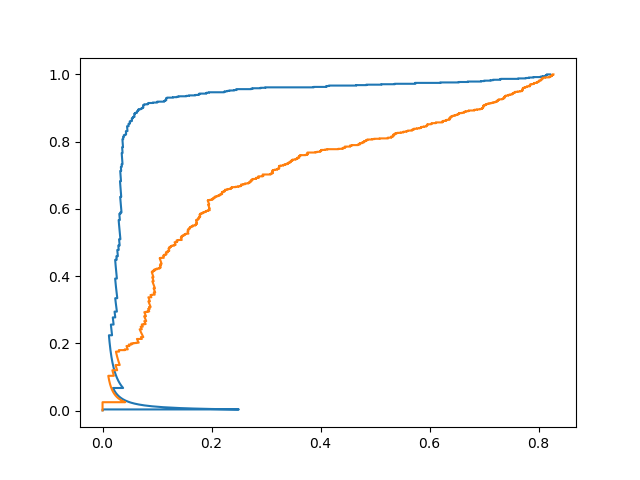
\includegraphics[width=0.9\linewidth]{./figures/roc-microns-300-test.png}
	\caption{(NOT CORRECT) The receiver operating characteristic (ROC) curve for all four datasets.}
	\label{fig:network-results}
\end{figure}

TODO - ADD QUALITATIVE RESULTS

\subsection{Graph Based Strategies}

TODO - QUANTIFY IMPROVEMENT BY MULTICUT - READERS CAN SKIP SECTION FOR NOW

Using a graph-based optimization strategy prevents XX segments from merging compared to the simple hierarchical agglomeration strategy with an optimal threshold cut off. Since correcting merge errors is significantly more difficult than correcting split errors, it is desirable to limit the number of false merges. The graph-based strategies significantly improve this error type. 

\subsection{Variation of Information Improvements}

We compute the variation of information for our segmentations against the expert-labeled ground truth datasets. 
The input segmentation to our network serves as a baseline. 
We evaluate NeuroProof (our input) at several different thresholds to create a variation of information curve. 
Similarly, we run the greedy-additive heuristic with varying parameters that increase the probability needed for merging nodes. 
Figure \ref{fig:variation-of-information} shows the results on the datasets compared to the baseline (green) and an oracle (blue). 
The oracles sees the entire constructed graph from our algorithm and correctly partitions the graph based on the ground truth. 
Our methods decreases the split variation of information by a factor of XX\% and only increases the merge variation of information by a factor of XX\% on the test datasets. 
Table \ref{table:variation-of-information} provides a quantitative overview for the changes in variation of information.

TODO - ADD QUALITATIVE RESULTS

\begin{table}
	\centering
	\begin{tabular}{c c c} \hline
		\textbf{Dataset} & \textbf{VI Split} & \textbf{VI Merge} \\ \hline
		Kasthuri Training &  & \\
		Kasthuri Testing & & \\
		FlyEM Vol. 1 & & \\
		FlyEM Vol. 2 & & \\ \hline
	\end{tabular}
	\caption{Variation of Information Change}
	\label{table:variation-of-information}
\end{table}


\begin{figure*}[t!]
	\centering
	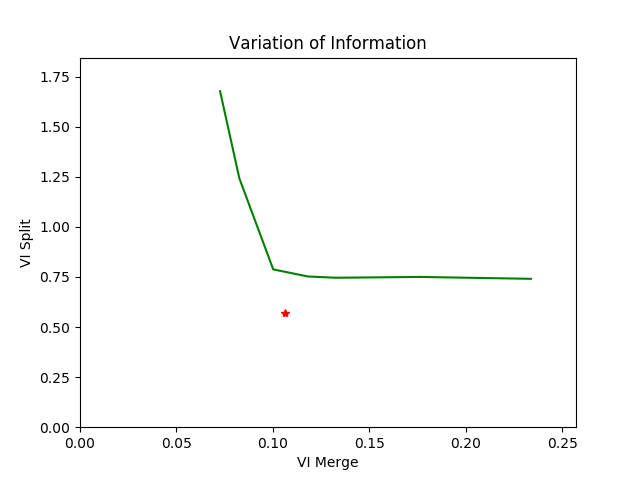
\includegraphics[width=0.42\linewidth]{./figures/variation_of_information-train.png}
	\hspace{0.085\linewidth}
	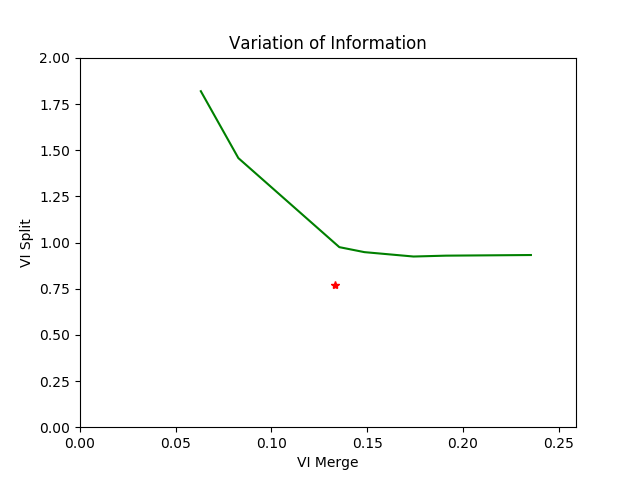
\includegraphics[width=0.42\linewidth]{./figures/variation_of_information-test.png}
	\caption{The improvement on variation of information from the baseline NeuroProof segmentation (green). Results closer to the origin are better.}
	\label{fig:variation-of-information}
\end{figure*}